%!TeX root=../tese.tex
%("dica" para o editor de texto: este arquivo é parte de um documento maior)
% para saber mais: https://tex.stackexchange.com/q/78101

\chapter{Metodologia}

% falar sobre validação cruzada
% falar que foi em python, libs, 
% dados amostrados ao longo do tempo => não misturamos 
% validação cruzadas 
% n modelo => falar melhores

% melhorar.. só usar isso?
Neste trabalho, utilizou-se dados públicos de fontes como o Instituto Brasileiro 
de Geografia e Estatística (IBGE), a Fundação Getúlio Vargas, FGV, e o 
Banco Central do Brasil (BACEN) para prever o consumo mensal de 
cimento nos estados da União. Para melhorar o desempenho dos modelos de 
aprendizado de máquina, realizaram-se técnicas
de preparação de dados, como o preenchimento de valores nulos, e para mensurar 
o acerto das previsões são aplicadas as métricas estatísticas: \textit {root 
mean squared error} (RMSE),  \textit{mean absolute error} (MAE) e \textit{mean 
absolute percentage error} (MAPE), além da variação percentual.


\section{Dados}
\label{sec:dados}

O consumo mensal de cimento nos estados do Brasil, alvo da previsão 
dos modelos aplicados neste trabalho, é um indicador fornecido pelo SNIC, 
Sindicato Nacional da Indústria de Cimento. Os dados obtidos apresentavam granularidade
mensal para cada um dos estados da União e estavam disponíveis de 1990 até 2021,
a exceção dos anos de 2001 e 2002. Dessa forma, optou-se por utilizar apenas 
dados posteriores a 2003 no trabalho, uma vez que os modelos recorrentes se 
valem do contexto para obter a próxima previsão \ref{rnn} , então esse lapso nos dados
poderia trazer inconsistências no modelo.

Além disso, o descarte de dados mais antigos favorece a assertividade do 
modelo, pois houve alteração no total de cimento consumida no Brasil
ao longo do tempo, então dados mais antigos poderiam privilegiar tendências 
mais antigas. Retirar dados mais antigos, então evita, por exemplo, que a 
estagnação econômica da época de hiperinflação ou o otimismo do Plano real
impacto a previsão atual. Essa alteração na quantidade de cimento consumida pela União
pode ser observada na imagem abaixo. 

\begin{figure}[H] 
    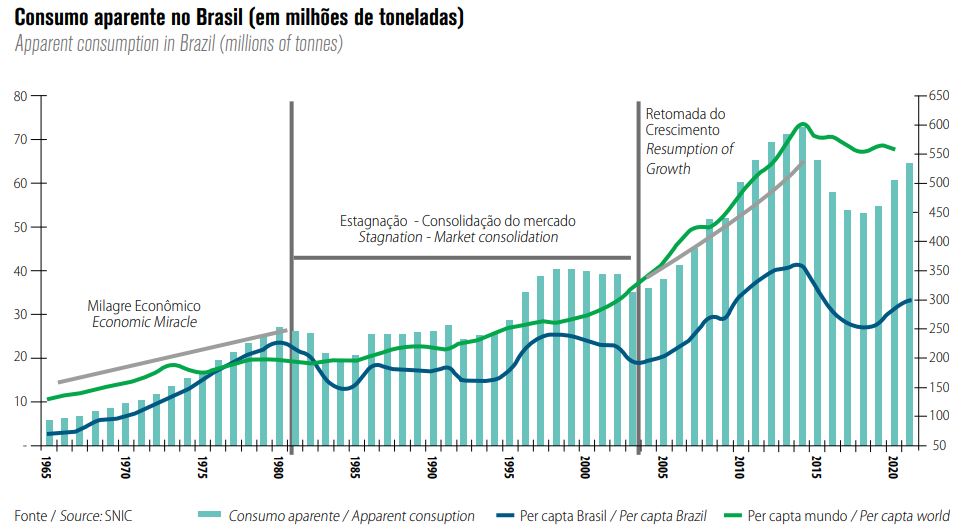
\includegraphics[width= 14cm]{../figuras/evolucao-consumo.png}
    \caption{Evolução do consumo de cimento no Brasil \cite{relatorio-snic}}
    \label{fig:evolucao-consumo-cimento}
\end{figure}

Observa-se, por exemplo, uma queda no consumo de cimento entre 2015 e 2018,
fruto das crises econômicas nesse período. Ressalta-se, também,
que o consumo não é uniforme ao longo do ano como pode ser 
visto na figura \ref{consumo-sp}, aonde bserva-se a 
grande variação na demanda de cimento no estado
de São Paulo, não apenas ao longo dos anos, mas também ao 
longo dos meses do ano

\begin{figure}[H]
    \centering
    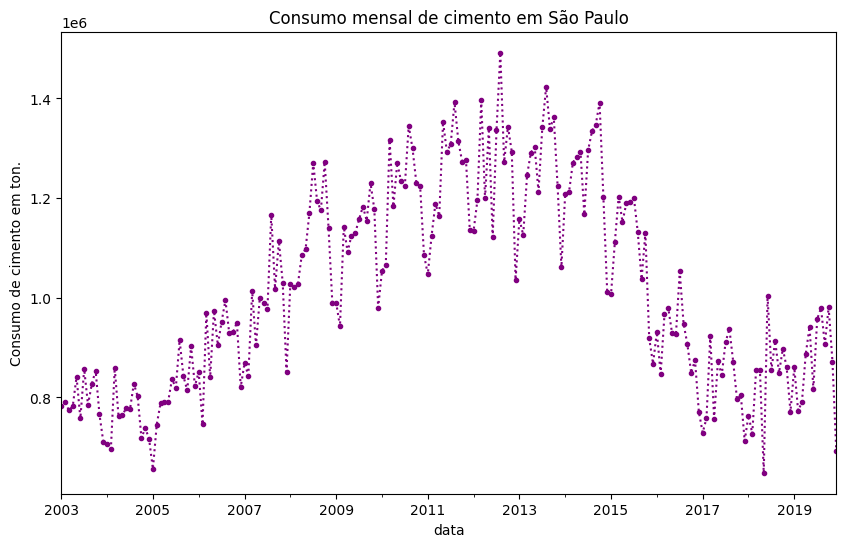
\includegraphics[width=10cm]{../figuras/graficos/evolucao-consumo-sp.png}
    \caption{Evolução do consumo mensal de cimento em São Paulo}
    \label{consumo-sp}
\end{figure}

Além disso, destaca-se que existe uma 
grande diferença no consumo entre os estados do Brasil, por 
exemplo, o consumo médio em São Paulo de 2003 a 2019 foi de 
aproximadamente 1014,7 mil toneladas enquanto o de 
Alagoas foi de 41,5 mil toneladas. Mesmo ao comparar apenas
estados de uma mesma região, é evidente que há singularidades 
de cada unidade da federação, como pode ser visto na imagem
\ref{consumo-se}.

\begin{figure}[H]
    \centering
    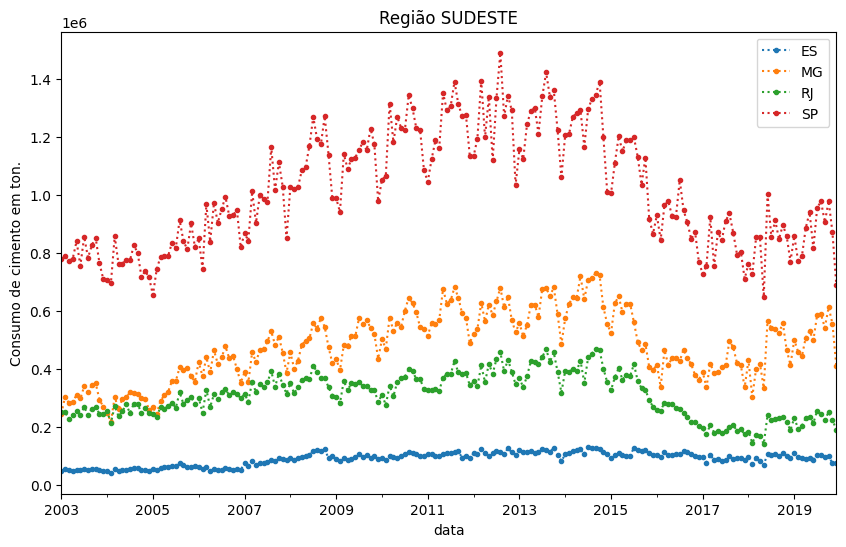
\includegraphics[width=10cm]{../figuras/consumo/dado-se.png}
    \caption{Evolução do consumo de cimento nos estados do Sudeste}
    \label{consumo-se}
\end{figure}

No gráfico \ref{consumo-se}, os pontos representam cada uma das
 medições mensais  do consumo de cimento em cada um dos estados
 da região.

A região Sudeste foi escolhida neste trabalho para demonstrar as 
previsões do modelo. Essa escolha se deu pois possui apenas quatro 
estados, então o gráfico com as previsões é mais simples de 
ler e interpretar que o de outras regiões com maior número de estados.
Além disso, os estados dessa região apresentam certa distância
na quantidade de cimento consumida, dessa forma, há pouca sobreposição 
entre as curvas, isso torna o gráfico mais legível também. Por 
exemplo, a média de consumo de cimento do período analisado no 
estado de São Paulo foi de 1014,7 mil toneladas, no Rio de Janeiro
foi de 310,2 mil toneladas, já em Minas Geral foi de 480,3 mil 
tonelada e no Espírito Santo, por sua vez, foi de 91,9 mil toneladas.

O modelo utiliza dados econômicos, sociais e da construção
civil para treinar estimar a demanda por cimento. Na tabela
\ref{tab:indicadores}, estão
apresentadas a fonte, granularidade e o período em que os dados 
estavam disponíveis para todos os indicadores utilizados neste 
trabalho. Na tabela são utilizadas siglas para melhor visualização,
como IBGE para Instituto Brasileiro
de Geografia e Estatística, FGV para Fundação Getúlio Vargas,
BACEN para Banco Central do Brasil, IPEA para Instituto de 
Pesquisa Econômica Aplicada e SNIC para Sindicato Nacional 
da Indústria do Cimento todas fontes utilizadas neste trabalho.
Além disso, utilizou-se abreviação para Produto Interno Bruto (PIB),
Índice Nacional de Preços ao Consumidor Amplo (IPCA),
Índice Nacional de Custo da Construção (INCC), Índice Geral de 
Preços (IGP), Necessidade de Financiamento do Setor Público (NFSP) e 
Índice de Desenvolvimento Humano (IDH).


\begin{table}[H]
    \centering
    \caption{Indicadores utilizados no trabalho}
    \begin{tabular}{llll}
        \toprule
        Indicador                   & Fonte & Período disponível & Granularidade         \\
        \midrule
        PIB a preços constantes     
                                    & IBGE\footnote{\label{portal ipea} Dado retirado do portal do Ipeadata em \url{http://www.ipeadata.gov.br/Default.aspx}}  & 1983 até 2019      & anual por estado      \\
        PIB a preços de mercado      & IBGE\footref{portal ipea}  & 1985 ate 2019      & anual por estado      \\
        PIB per capita              & IBGE\footref{portal ipea}  & 1985 até 2019      & anual por estado      \\
        PIB da construção civil      & IBGE\footref{portal ipea}  & 1985 até 2019      & anual por estado      \\
        Desemprego                   & IBGE\footref{portal ipea}  & 1991 até 2022      & irregular \footnote{Havia dados de 1992 até 2014
        com granularidade anual e por estado, contudo, a partir de 2012 foram disponibilizados dados mensais a nível de Brasil por conta da 
        Pesquisa Nacional por Amostra de Domicílios (PNAD) Contínua mensal realizada pelo IBGE. Neste trabalho, utilizou-se os dados anuais até 2012
        e, após 2012, os dados provenientes da PNAD Contínua} \\
        IPCA                        & IBGE\footnote{Dado retirado do IBGE em \url{https://sidra.ibge.gov.br/tabela/1737}}  & 1981 até 2021      & mensal para o Brasil      \\
        INCC                        & FGV\footnote{Dado obtido a partir do portal da FGV em \url{https://www.debit.com.br/tabelas/tabela-completa-pdf.php?indice=incc}}   & 1980 ate 2021      & mensal para o Brasil      \\
        IGP                         & FGV\footref{portal ipea}   & 1944 até 2021      & mensal para o Brasil      \\
        Taxa Selic                  & IBGE\footnote{Dado obtido em \url{https://www.debit.com.br/tabelas/tabela-completa.php?indice=selic}}  & 1986 até 2022      & mensal para o Brasil      \\
        NFSP                        & BACEN\footref{portal ipea}  & 1991 até 2022      & mensal para o Brasil      \\
        Estoque líquido de capital fixo   & IPEA\footref{portal ipea}   & 1947 ate 2019      & anual para o Brasil      \\
        População                   & IBGE\footnote{Dado obtido do portal Base dos Dados em \url{https://basedosdados.org/dataset/br-ibge-populacao}}   & 1991 até 2021      & anual por estado      \\
        IDH                         & IBGE\footref{portal ipea}   & 1991 ate 2017      & irregular\footnote{Os indicadores de IDH (Renda, Longevidade e Educação) estão disponíveis em anos de censo do IBGE (1990, 2000, 2010), há 
        dados, também, de 2014 a 2017 por conta da PNAD Contínua}      \\
        Produção mensal de cimento  & SNIC\footnote{\label{cbic} Dados retirados do portal \url{http://www.cbicdados.com.br/menu/materiais-de-construcao/cimento}}  & 2003 até 2022      & mensal por estado      \\
        Valor médio do cimento\footnote{Evolução do valor médio/mediano do cimento Portland 32 em US\$/Tonelada}      & IPEA\footref{cbic}   & 1947 ate 2019      & anual para o Brasil      \\
        \bottomrule
    \end{tabular}
    \label{tab:indicadores}
\end{table}
% quem sabe por a legenda no apendice

Com o objetivo de direcionar a estratégia de preparação de dados
foi realizada uma análise exploratória de cada um dos dados de 
entrada e da variável resposta. 
A partir dessa análise, 
optou-se por utilizar os dados de 2003 até 2019 para o estudo.
Destaca-se nessa análise, a alta
taxa de variação dos dados de entrada, em alguns indicadores, por exemplo 
para o  PIB da construção civil,   
o desvio padrão é maior que o valor médio do indicador. Dessa 
forma, está presente nos dados um grande número de \textit{outliers},
em especial ao analisar o Brasil como um todo, por conta da 
forte diferença entre as regiões do Brasil. 

\begin{quote}
    \textit{An outlier is an observation strikingly far from
some central value. It is an unusual value relative
to the bulk of the data...}\cite{tukey77}
\end{quote}

\textit{Outliers} são observações discrepantes do restante dos dados, que parecem
inconsistentes e podem interferir no processo de previsão. \cite{outliers}
Para ilustrar melhor o alto volume de \textit{outliers} presentes
nos dados, utilizou-se gráficos \textit{boxplot}, como mostrado na 
figura abaixo.

\begin{figure}[H]
    \centering
    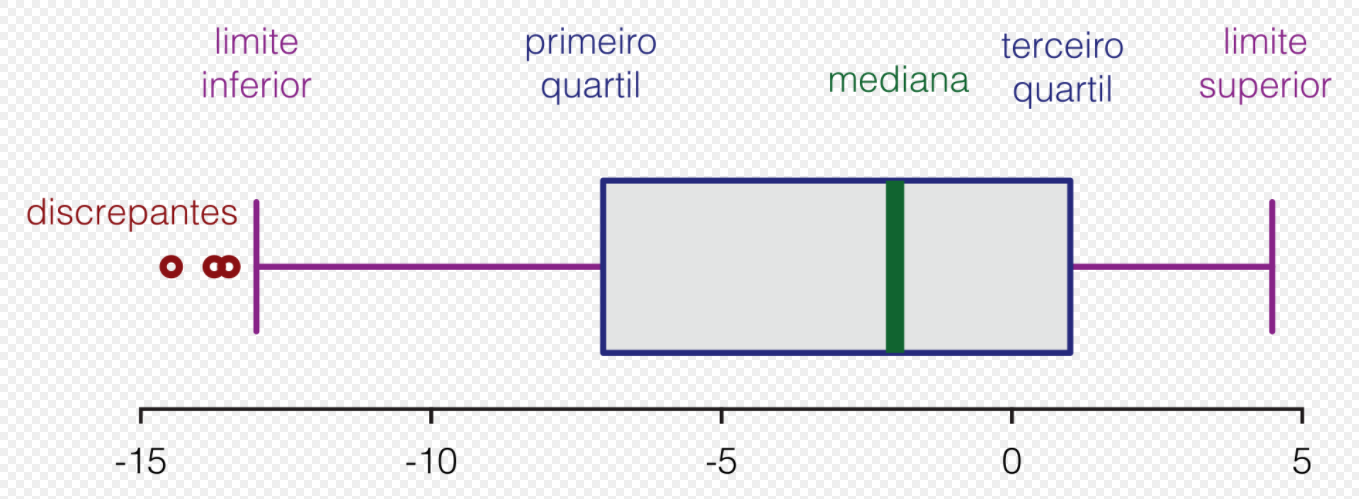
\includegraphics[width=8cm]{../figuras/explicacao-boxplot.png}
    \caption{Gráfico \textit{boxplot} \cite{explicacao-boxplot}}
    \label{fig:boxplot}
\end{figure}

O \textit{boxplot} \cite{boxplot} é
uma técnica estatística utilizada na análise exploratória
os dados para identificar visualmente padrões, como a distribuição
dos dados. Na figura, acima linha em verde corresponde à mediana \footnote{
valor que fica no meio quando os dados estão ordenados ou a média
dos dois valores centrais se o número de pontos de dados for par
\cite{boxplot-stat}} 
dos dados, os limite inferior e o superior ao retângulo representam
o primeiro e terceiro quartil\footnote{O primeiro e terceiro 
quartis também representam a mediana dos valores superiores
à mediana dos dados e a mediana dos valores inferiores à mediana. Então metade
dos dados está contida dos quadrados nas imagens}, respectivamente. 

\begin{figure}[H]
    \centering
    \label{fig:boxplot_all}
    \begin{subfigure}{5 cm}
        \centering
        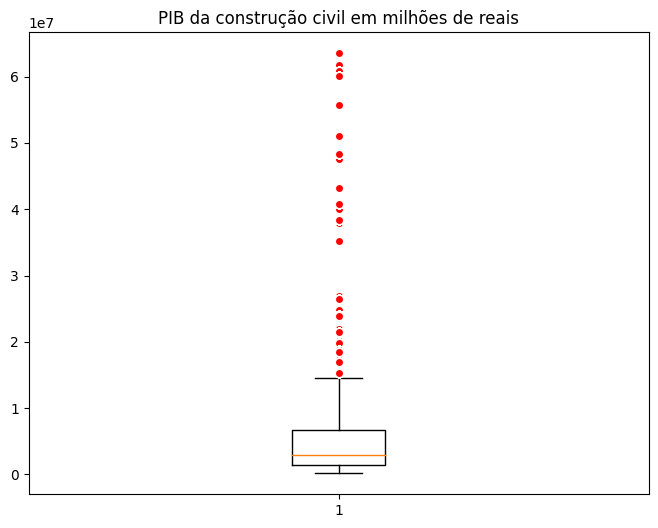
\includegraphics[width=5cm]{../figuras/graficos/boxplot-pib-cc.png}
        \caption{Gráfico \textit{boxplot} do Brasil}
    \end{subfigure}
    \hfill
    \begin{subfigure}{5cm}
        \centering
        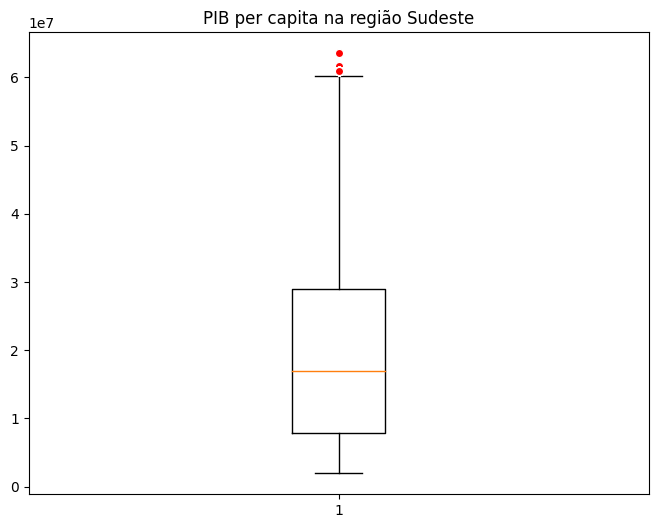
\includegraphics[width=5cm]{../figuras/graficos/boxplot-pib-cc-se.png}
        \caption{Gráfico \textit{boxplot} do Sudeste}
    \end{subfigure}
    \hfill
    \begin{subfigure}{5cm}
        \centering
        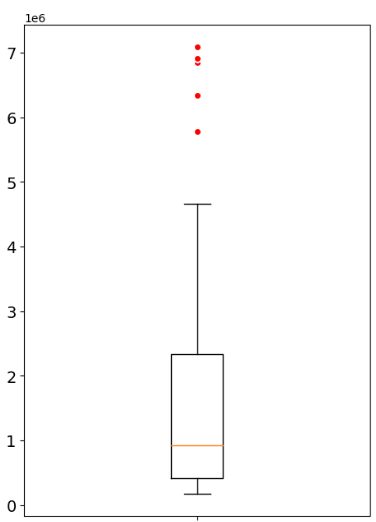
\includegraphics[width=4.8cm]{../figuras/graficos/boxplot-pib-cc-n.png}
        \caption{Gráfico \textit{boxplot} do Norte}
    \end{subfigure}
\end{figure}

Conforme explicado na figura \ref{fig:boxplot}, a linha em 
laranja nos gráficos acima representa a mediana dos dados,
o retângulo que envolve a mediana é delimitado pelo primeiro e 
terceiro quartil e retém metade central das amostras. Os valores
reoresentados por pontos vermelhos acima ou abaixo dos limites
superiores ou inferiores são \textit{outliers}. Observa-se,
então, que pode-se obter uma significativa redução no número de 
amostras com \textit{outliers} ao separar a análise por região.\cite{boxplot}

Analisou-se, também, a correlação entre as variáveis de entrada e observou-se
alta correlação entre os indicadores de PIB do estado, PIB da construção
civil e população. Além disso, há alta correlação entre os três indicadores
de IDH, além do preço do saco de cimento e o preço do kilograma, como pode-se
validar na figura \ref{fig:matriz-corr}.

\begin{figure}[H]
    \centering
    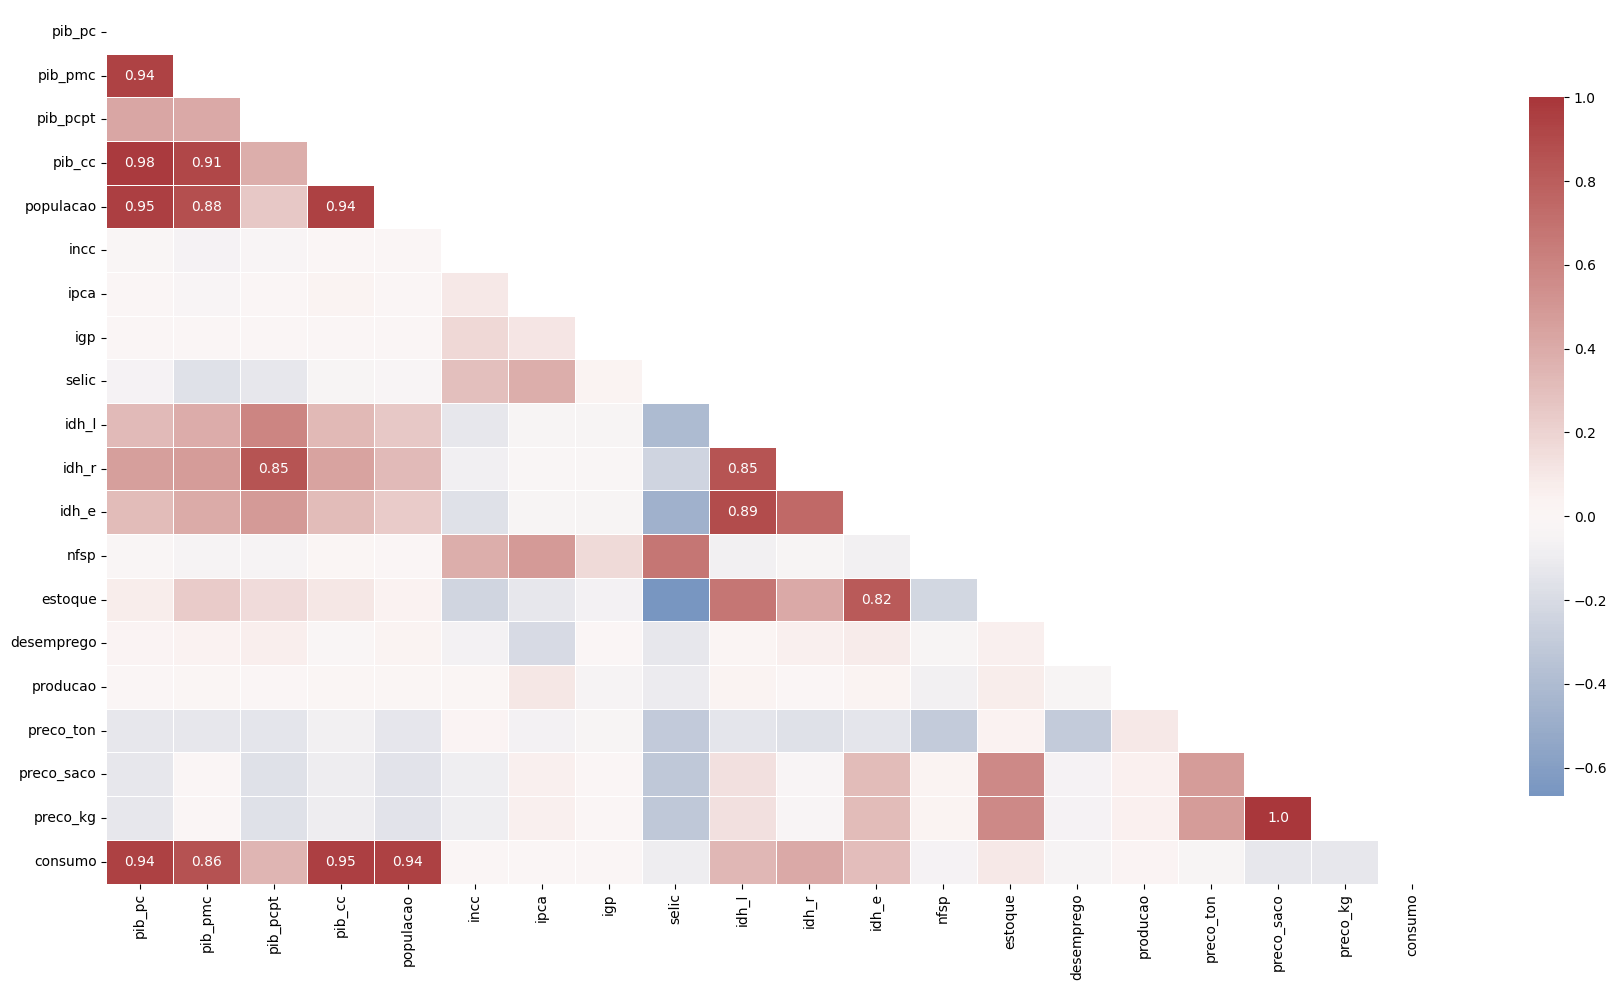
\includegraphics[width=13cm]{../figuras/graficos/matriz-corr.png}
    \caption{Matriz de correlação}
    \label{fig:matriz-corr}
\end{figure}

Foram adotadas estratégias para garantir dados na granularidade
mensal e por estado. Caso os indicadores apresentassem granularidade anual, 
o valor foi dividido por 12 de modo a obter a média mensal, já caso a granularidade
fosse a nível de Brasil, o valor apresentado foi repetido para todos os 
estados.


A estratégia utilizada para lidar com dados faltantes foi, sempre que possível,
repetir o valor anterior que estava disponível nos dados de entrada para
preencher a ocorrência. Contudo, alguns indicadores não apresentavam 
valores mais antigos, então foi usado um valor não presente no intervalo
de dados de entrada (-1) para marcar como nulo. Os indicadores 
com dados faltantes são, em ordem descrescente de acordo com 
o percentual de dados faltantes: produção de cimento, valor 
médio do quilo, saco e da tonelada e cimento e desemprego.

Além disso, tomou-se um cuidado para evitar que a previsão fosse 
realizada com os dados do mês anterior ou do ano anterior no caso dos
indicadores anuais. Deslocou-se, portanto, os dados de entrada 
para frente em um ocorrência de modo a associar os dados de um 
mês com o consumo no mês seguinte.\footnote{os dados correspondentes 
a, por exemplo, fevereiro de 2004 estão relacionados ao consumo de 
cimento em março de 2004, com o objetivo de propor um cenário mais pertinente, 
uma vez que o objetivo do projeto é prever a demanda por cimento no mês seguinte 
em um estado a partir dos dados do mês atual e, eventualmente, dos anteriores.
}

Por fim, o estado correspondente à medição foi usado como dado de entrada. 
Como os modelos de inteligência artificial aceitam apenas caracteres numéricos,
utilizou-se o método de codificação \textit{one hot} para criar 27 colunas, uma
para cada estado, nas quais o valor é 1 quando a linha possui dados daquele estado 
e é 0 caso contrário.


    \section{Avaliação de performance}

    Para comparar a eficiência dos modelos mede-se os erros de 
    cada previsão, ou seja, a distância entre o valor previsto 
    pelo algoritmo e o valor do dado real. Neste trabalho, 
    utilizou-se as seguintes métricas estatísticas para 
    mensurar o desempenho: \textit{mean absolute error} (MAE),
    \textit{root mean square  error} (RMSE) e \textit{mean 
    absolute percentage error} (MAPE). Além disso, foi utilizado
    o delta percentual ($\Delta$) para avaliar se o modelo tende 
    a subestimar ou superestimar o valor previsto, se é otimista
    ou pessimista.

\subsection{Mean absolute error (MAE)}

    O MAE, sigla do inglês para \textit{mean absolute error}
    ou média do erro absoluto mede o erro absoluto de cada previsão
    e é dado por:\cite{forecast-evaluation-ds}

    \begin{equation}
        MAE = \frac{\sum_{i=1}^n |\hat{y}_i - y_i|}{n}
    \end{equation}

\subsection{Root mean squared error (RMSE)}

    A RMSE, sigla para \textit{root mean squared  error} é
    semelhante à MAE, contudo eleva os erros ao quadrado antes de 
    somá-los e tira a raiz logo depois. A RMSE é, portanto, 
    mais sensível a \textit{outliers}.\cite{forecast-evaluation-ds}

    \begin{equation}
        RMSE = \sqrt{\frac{\sum_{i=1}^n (\hat{y}_i - y_i)^2}{n}}
    \end{equation}

\subsection{Mean absolute percentage error (MAPE)}

    Foi utilizada também a MAPE, \textit{Mean absolute
    percentage error}, para mensurar a escala do erro em 
    relação ao tamanho das medições.

    \begin{equation}
        MAPE=\sum_{t=1}^n\left|\frac{y_t-\hat{y}_t}{y_t}\right|
    \end{equation}

\subsection{Delta percentual}

O delta percentual, $\Delta$, é utilizado para mensurar se o 
modelo apresenta tendência de subestimar ou superestimar a variável, se 
é otimista ou pessimista.

\begin{equation}
    \Delta = \frac{\hat{y_i} - y_i}{y_i}
\end{equation}